\section{Introduction}

Solving partial differential equations (PDEs) underpins critical scientific advancements across diverse fields. The current approach to solving a PDE relies almost entirely on the prominent tool named FEniCSx, traditionally involving the specification of input parameters \footnote{Typically the input parameters include the materials parameter, the boundary conditions and the geometric parameter}, coding the problem, and utilising the finite element method(FEM) and the FEniCSx framework to obtain a solution manifold. 

This project proposes an alternative approach to solving PDEs by integrating Model Order Reduction (MOR) with Neural Networks (NN). The method involves reducing input order through MOR (with the RBniCSx package), training the NN with snapshots of PDE solutions as inputs, and using the pre-trained model for efficient PDE solving. While offering data-driven efficiency and reducing reliance on tools like FEniCSx, there are trade-offs, including a sacrifice in accuracy and extended training times for the neural network. Striking a balance between accuracy and efficiency is crucial for the successful implementation of this hybrid approach in scientific computing.

To accelerate the training of our Neural Network, this project leverages supercomputers through parallel computing, which divides tasks into smaller batches, allowing multiple processors to concurrently execute computations. In the context of NN training, data batches are distributed to individual processors, each handling its own subset. Through forward and backward passes, as well as weight optimization, parallel processing accelerates the training process. In the meanwhile, the outputs during each training epoch (e.g. losses and gradients) are also synchronised among processors, as shown in figure \ref{fig: parallel}. The process is facilitated by a designated communicator. This parallelization is implemented using TensorFlow for GPU-based NN training and also extends to CPU-based parallel computing, particularly in the context of solving large-scale PDEs with FEniCSx.

\begin{figure}[!h]
        \begin{center}
	\begin{subfigure}{0.35\linewidth}
		\centering
		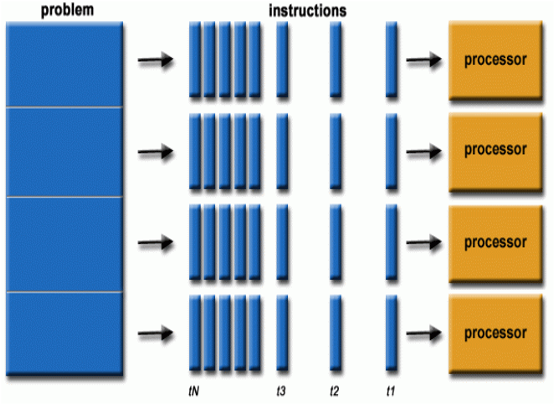
\includegraphics[width=\linewidth]{figs/parallel1.png}
	\end{subfigure}
	\begin{subfigure}{0.35\linewidth}
		\centering
		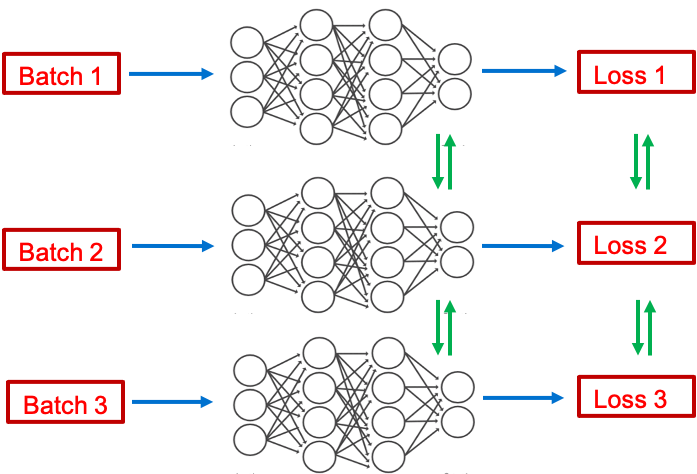
\includegraphics[width=\linewidth]{figs/parallel2.png}
	\end{subfigure}
	\caption{Parallel computing and its application in training an NN}
	\label{fig: parallel}
        \end{center}
\end{figure}